\section{Introduction}
\begin{itemize}
  \item Motivation: theoretical possibility of high energy recoil events. Mention some specific models, maybe inelastic scattering also.
  \item Theoretical background on EFT operators.
  \item (if we do it) Theoretical background on inelastic scattering kinematics.
  \item Motivating example plots of recoil spectra/signal models (e.g. Fig. \ref{fig:dRdE}). Also discuss the lower electronic recoil background at these higher recoil energies, which improves the analysis sensitivity beyond what would be expected from the raw increase in predicted event rate (At least I presume so, need to estimate this perhaps. I think we can say something like this; the standard analysis signal region has a signal acceptance of maybe 50\% since it cuts the nuclear recoil band about in half, whereas for us it is almost 90\% since there is good separation between ER and NR bands. So for say O3 (either mass) we expect about twice as many events due to the extended signal region, with twice the acceptance in the new high PE region. So overall I guess it is roughly a factor of 3 improvement in total signal rate, and similar for the sensitivity. In fact from the proper sensitivity estimates the improvement is a little better than that, but this gives a rough idea where the improvement comes from.).

\begin{figure}[h!]
\begin{minipage}{1.\linewidth}
\centerline{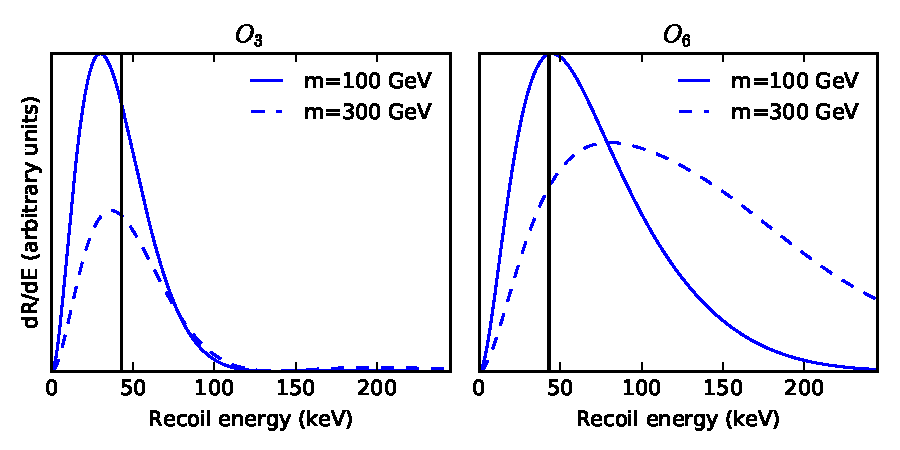
\includegraphics[width=1.\linewidth]{Figures/dRdE_examples.pdf}}
\end{minipage}
\caption{Example EFT recoil spectra for elastic scattering of spin-$1/2$ WIMPs on Xenon nuclei (weighted according to the isotope abundances in the XENON100 experiment). Left(right) shows the predicted spectra for EFT operate $O_3$($O_6$). The normalisation is controlled by the coupling coefficient of each EFT operator and the experimental exposure (left arbitrary in this figure). The solid vertical line at 43 keV shows the approximate division between the two signal regions used in this analysis (30 PE in cS1). As shown, certain EFT operators, for certain WIMP masses, predict a significant fraction of recoil events above the upper energy cut used in the standard spin-independent analysis, motivating an extension of this cut.}
\label{fig:dRdE}
\end{figure}


\end{itemize}
\section{The \Xehund\  Detector}
The \Xehund\ detector is a cylindrical (30cm height X 30cm diameter) dual phase Xenon Time Projection Chamber (TPC) that holds 62 kg of Liquid \Xe\ (LXe) targets ~\cite{xe100_instr2012}. It operates at the Laboratori Nazionali del Gran Sasso (LNGS) in Italy. The detector consists a total of 242 1”-square Hamamatsu R8520-AL photomultiplier tubes (PMTs) employed in two arrays, at the top part (in the gas phase) and in the bottom immersed in LXe. a Particle interacting with the LXe deposits energy that creates both excited and ionized states. De-excitation creates a prompt scintillation signal ($S1$). ,  Ionized electrons are drifted in an electric field of $530$V/cm towards the liquid-gas interface, where they are extracted via a larger electric field of $\sim12$kV/cm. These electrons generates a proportional scintillation, which is called $S2$. The spatial distribution of the $S2$ signal on the top PMT array, determines the X-Y position, while the time difference between the two signals gives the z-coordinate, and thus a 3D position reconstructions is achieved.

The ratio of S2/S1 is different weather the interaction is nuclear recoil (NR) or electronic recoil (ER) and thus this ratio is used as a discriminator between ER background coming from $\gamma$, $\beta$ and NR signal coming from a WIMP. 

In previous \Xehund\ analyses the determination of the recoil energy was based on the size of S1 and the scintillation efficiency for the nuclear recoils, \Leff ~\cite{xe100_run10_si}. However in the last analysis ~\cite{xe100_run_combination} a new method was adopted taking into advantage also the S2 signal.
      

